\documentclass[11pt]{article}
\usepackage[margin=1in]{geometry}
\usepackage[utf8]{inputenc}
\usepackage[T1]{fontenc}
\usepackage{lmodern}
\usepackage{amsmath,amssymb}
\usepackage{graphicx}
\usepackage{booktabs}
\usepackage{xcolor}
\usepackage[hidelinks]{hyperref}
\usepackage{url}
\usepackage{caption}
\usepackage{listings}
\usepackage{tikz}
\usetikzlibrary{arrows.meta,positioning,fit,calc}
\captionsetup{font=small,labelfont=bf}

\definecolor{ink}{HTML}{0B0B0B}
\definecolor{muted}{HTML}{52514E}
\definecolor{pblue}{HTML}{2A78D6}
\definecolor{porange}{HTML}{EB6834}
\definecolor{paqua}{HTML}{1BAF7A}
\definecolor{codebg}{HTML}{F6F5F2}

\lstset{basicstyle=\ttfamily\footnotesize, columns=fullflexible, keepspaces=true, frame=none,
  backgroundcolor=\color{codebg}, xleftmargin=1em, aboveskip=0.6em, belowskip=0.6em, language=C++,
  keywordstyle=\color{ink}\bfseries, commentstyle=\color{muted}\itshape, showstringspaces=false,
  morekeywords={__global__,__device__,__shared__}}

\newcommand{\memprint}{MemPrint}
\newcommand{\secref}[1]{Section~\ref{#1}}
\newcommand{\figref}[1]{Figure~\ref{#1}}
\newcommand{\tabref}[1]{Table~\ref{#1}}
\newcommand{\term}[1]{\emph{#1}}
\newcommand{\code}[1]{\texttt{#1}}

\title{Finding the Memory Dependences Between GPU Kernels\\by Interpreting the Program's CUDA Source}
\author{Nafis Mustakin\\University of California, Riverside}
\date{October 2026}

\begin{document}
\maketitle

\newcommand{\numPrograms}{13}
\newcommand{\numMustTotal}{1{,}650}
\newcommand{\numCcRecall}{0.98}
\newcommand{\numCcRecallLo}{0.981}
\newcommand{\numCcRecallHi}{0.995}
\newcommand{\numCcMissLo}{0.5\%}
\newcommand{\numCcMissHi}{1.9\%}
\newcommand{\numCcMustRecallLo}{0.36}
\newcommand{\numCcMustRecallHi}{0.45}
\newcommand{\numCcLockPrecLo}{0.76}
\newcommand{\numCcLockPrecHi}{0.92}
\newcommand{\numCcLockFalseLo}{8\%}
\newcommand{\numCcLockFalseHi}{24\%}
\newcommand{\numCcPlain}{50}
\newcommand{\numCcReps}{10}
\newcommand{\numCcGpuRuns}{60}
\newcommand{\numCcGpuRoundsLo}{20}
\newcommand{\numCcGpuRoundsHi}{24}
\newcommand{\numCcInterpRoundsLo}{13}
\newcommand{\numCcInterpRoundsHi}{24}
\newcommand{\numDataDeps}{1{,}427}
\newcommand{\numDataMust}{1{,}032}
\newcommand{\numBfsDeps}{868}
\newcommand{\numPtrselNoSplitMust}{18}
\newcommand{\numNoInputPatterns}{15}
\newcommand{\numNoInputPatternsOf}{22}
\newcommand{\numOverheadLo}{0.3}
\newcommand{\numOverheadHi}{624}
\newcommand{\numKernelRatioLo}{0.05}
\newcommand{\numKernelRatioHi}{11.5}
\newcommand{\numKernelRatioMedian}{0.6}
\newcommand{\numScheduleCost}{17.2}
\newcommand{\numScheduleLo}{3.9}
\newcommand{\numScheduleHi}{94}
\newcommand{\numNvbitLo}{2.0}
\newcommand{\numNvbitHi}{13.8}
\newcommand{\numNativeLo}{0.31}
\newcommand{\numNativeHi}{0.37}
\newcommand{\numChainThreads}{3{,}000{,}448}
\newcommand{\numChainKernelS}{4.0}
\newcommand{\numRbfsThreads}{2{,}228{,}224}
\newcommand{\numRbfsLockS}{2.8}
\newcommand{\numRbfsNvbitS}{2.2}
\newcommand{\numWlbfsLockS}{214}
\newcommand{\numWlbfsKernelS}{0.24}
\newcommand{\numBfsLockS}{122}
\newcommand{\numBfsKernelS}{0.8}
\newcommand{\numHostShareMax}{99.9\%}


\begin{abstract}
A CUDA program runs as a sequence of operations on the GPU: kernel launches, copies between host and device
memory, and memory fills. One operation depends on an earlier one when it reads bytes the earlier one wrote, or
writes bytes the earlier one read or wrote. A runtime system that knows these dependences can run independent
operations at the same time, reorder them, or place their data, but in graph programs and other irregular code the
bytes a kernel touches are chosen by values in memory, such as the neighbour lists of a graph, so a compiler cannot
determine them from the source code. We present an interpreter that runs the program's CUDA source, host code and
kernels together, on the CPU with the program's real input, and records which bytes every operation reads and
writes. The interpreter runs all the threads of a kernel at once as arrays, one statement at a time, so a value
loaded from memory, a branch on such a value, and an address computed from it are all known exactly. Two further
mechanisms handle cases that a single run in this form would get wrong. When the threads of a kernel load
pointers that name different buffers, the interpreter splits the threads into groups by buffer and runs each group
separately. When the bytes a kernel touches depend on the order in which threads run, the interpreter runs the
program under four legal thread orders and reports a dependence as certain only if every order produces it. We
compare the interpreter against the bytes each operation actually touched on an NVIDIA A30 GPU, recorded with an
NVBit tool we built for the purpose, on \numPrograms{} test programs that include three breadth-first searches,
a connected-components kernel and kernels that choose buffers through tables of pointers. Every dependence the
interpreter reports as certain occurs on the GPU (\numMustTotal{} certain dependences, none wrong), and the
interpreter finds every dependence of 12 of the 13 programs. On connected components, where \numCcGpuRuns{} runs
on the GPU took \numCcGpuRoundsLo{} to \numCcGpuRoundsHi{} rounds and every traced run touched different bytes, it
finds \numCcRecallLo{} to \numCcRecallHi{} of each run's dependences. Of the \numDataDeps{} dependences between kernels that pass through bytes chosen by data,
\numDataMust{} are reported as certain and all of those occur on the GPU. The cost is the interpreter's run time on
the CPU, which for the inputs we measured is \numOverheadLo{} to \numOverheadHi{} times the program's whole run on
the GPU. Most of that time goes to host loops that the interpreter runs one iteration at a time, and the kernels
alone take \numKernelRatioLo{} to \numKernelRatioHi{} times the whole GPU run. Running all four thread orders costs
\numScheduleCost{} times as much as lockstep alone, on average. The exact bytes depend on the input, so they can be known only once the input
is known, but the pattern of dependences between kernels was the same for three different graphs.
\end{abstract}

\section{Introduction}
\label{sec:intro}

A CUDA program is a host program, running on the CPU, that issues work to the GPU. The work arrives at the GPU as
a sequence of \term{operations}: a \term{kernel launch} runs a function, the kernel, on many GPU threads at once,
a \term{copy} moves bytes between host memory and device memory or within device memory, and a \term{fill}
(\code{cudaMemset}) sets a range of device memory to one value. By default the GPU runs these operations one
after another, in the order the host issued them. That order is always safe, but it is often slower than
necessary, because two operations that touch different bytes could run at the same time, and an operation whose
inputs are ready could start before an unrelated operation finishes. CUDA lets a program express such freedom with
streams and with task graphs~\cite{cudaguide}, and research systems schedule GPU work from a dependence graph
between kernels or parts of kernels~\cite{Abdolrashidi2017Wireframe,Abdolrashidi2021BlockMaestro}. All of these
need to know which operations depend on which.

An operation \emph{depends} on an earlier one when they touch the same bytes and at least one of them writes them.
For regular code, where every address is a simple function of the thread index and the sizes, a compiler can work
out the bytes each kernel touches from the source code alone~\cite{Feautrier1991Dataflow}. For irregular code it
cannot. In a graph program the addresses a kernel touches are read from memory. For example, a breadth-first search visits
\code{cost[edges[i]]}, where \code{edges} holds the graph, and it runs that statement only for vertices whose
entry in a frontier array is set, an array that the previous kernel wrote. Which bytes the kernel touches is
therefore a function of the input graph and of everything the program computed before the launch. Graph
benchmark suites for GPUs consist mostly of such kernels~\cite{Che2013Pannotia,Burtscher2012Irregular,Wang2016Gunrock}.

In this work we determine these dependences by running the program's source code on the CPU, with its input, in an
interpreter that records the bytes every operation touches. The interpreter extends \memprint{}'s interpreter for
C and C++ programs~\cite{memprintGeneralization}, which runs a program's syntax tree from \code{main()} and keeps
the values the program stores in memory, so that an address read from memory is known. We add the execution of
kernels, the bookkeeping that turns touched bytes into dependences, and two mechanisms that irregular GPU code
needs, and we measure the result against a GPU.

In this work, we make the following contributions:
\begin{itemize}
\item We describe an interpreter that runs a CUDA program's host code and kernels from source, runs all threads
of a kernel together as arrays, and reports for every pair of operations whether they depend on each other, through
which buffer, over how many bytes, and whether the dependence is certain or only possible (\secref{sec:interp}).
\item We show how to handle a kernel whose threads use different buffers chosen through pointers stored in
memory, by splitting the threads into groups by buffer (\secref{sec:split}), and a kernel whose touched bytes
depend on the order in which threads run, by running several legal thread orders and keeping as certain only what
they agree on (\secref{sec:schedules}).
\item We build an NVBit~\cite{Villa2019NVBit} tool that records the bytes each operation touches on a real GPU,
and a scoring method that compares two runs even when they issue a different number of operations
(\secref{sec:truth}).
\item We evaluate the interpreter on \numPrograms{} programs on an NVIDIA A30: every certain dependence it reports
occurs on the GPU, it finds all dependences in 12 of 13 programs, and it costs \numOverheadLo{} to
\numOverheadHi{} times the program's whole run on the GPU, most of it in host code (\secref{sec:eval}).
\end{itemize}

\section{Background and terms}
\label{sec:background}

This section defines the terms the rest of the paper uses. We assume only that the reader knows C.

\paragraph{Threads, blocks and kernels.} A kernel is a C++ function marked \code{\_\_global\_\_}. The host launches
it with a \term{grid} of $B$ \term{blocks}, each block a group of $T$ \term{threads}, and writes the launch as
\code{k<{}<{}<B,T>{}>{}>(\ldots)}. Every thread runs the whole function. A thread tells itself apart from the others through
the built-in values \code{blockIdx} and \code{threadIdx}, and usually computes from them the element it works on.
Threads of one block can share a small, fast memory (\code{\_\_shared\_\_} arrays) and wait for each other at a
barrier (\code{\_\_syncthreads()}). Threads of different blocks can communicate only through device memory, and
the order in which blocks run is not specified. An \term{atomic} operation, such as \code{atomicAdd(\&x, 1)},
reads and updates one memory location without another thread's update coming in between, and returns the old
value.

\paragraph{Operations and buffers.} We call every kernel launch, copy and fill an \term{operation}, and number
the operations in the order the host issues them. A \term{buffer} is one region of device memory obtained from
\code{cudaMalloc} or \code{cudaMallocManaged}. We measure memory in \term{units} of 4 bytes, so a dependence
through one \code{int} or \code{float} is one unit.

\paragraph{Dependences.} Operation $b$ depends on an earlier operation $a$ through a unit of a buffer if one of
three things holds. In a \term{read after write} (RAW), $a$ is the last operation before $b$ that wrote the unit,
and $b$ reads it, so $b$ needs the value $a$ produced. In a \term{write after write} (WAW), $b$ writes a unit that
$a$ was the last to write, so $b$ must not finish before $a$, or the final value would be $a$'s. In a \term{write
after read} (WAR), $b$ writes a unit that $a$ read after the last write, so $b$ must not overwrite it before $a$
has read it. We identify a dependence by its source operation, its destination operation, its kind and its buffer,
and we record over how many units it passes.

\paragraph{Certain and possible dependences.} A dependence is \term{certain} if the interpreter computed both accesses exactly,
and, when it ran the program under several thread orders (\secref{sec:schedules}), every order produced the
dependence. It is \term{possible} if at least one
of the two operations only perhaps touches it, for example because the access sits under a branch on a value the
interpreter does not know, or at an address it could not compute. A tool that consumes the dependences can rely on
a certain dependence, and must treat a possible one as present to stay safe.

\paragraph{Needed dependences.} If $c$ depends on $b$ and $b$ depends on $a$, then running the operations in an
order that respects the first two dependences also respects any dependence of $c$ on $a$. A scheduler therefore
needs only the dependences that are not implied by a path through others. In graph terms these form the
\term{transitive reduction} of the dependence graph, and we call them the \term{needed} dependences.

\paragraph{Indirect accesses and data-dependent branches.} An access is \term{indirect} if its address is computed
from a value loaded from memory, as in \code{a[b[i]]}. A branch is \term{data-dependent} if its condition reads
memory, as in \code{if (mask[tid])}. A dependence is \term{data-dependent} if it passes through units that were
touched by an indirect access or under a data-dependent branch. The interpreter marks these from the source code
(\secref{sec:events}). They are the dependences a compiler cannot determine, and the ones this paper is about.

\figref{fig:bfscode} shows both kinds in the kernel that expands the frontier in a breadth-first search, written
in the style of Rodinia's \code{bfs}~\cite{Che2009Rodinia}. Which threads pass the test on \code{mask[tid]},
which elements of \code{edges} they read, and which elements of \code{cost} and \code{updating} they write all
depend on the graph and on the previous levels of the search.

\begin{figure}[t]
\begin{lstlisting}
__global__ void expand(const Node *nodes, const int *edges, bool *mask, bool *updating,
                       const bool *visited, int *cost, int n) {
    int tid = blockIdx.x * blockDim.x + threadIdx.x;
    if (tid < n && mask[tid]) {                       // data-dependent branch
        mask[tid] = false;
        for (int i = nodes[tid].starting; i < nodes[tid].starting + nodes[tid].no_of_edges; i++) {
            int id = edges[i];                        // indirect: i comes from nodes[]
            if (!visited[id]) {                       // indirect, and a data-dependent branch
                cost[id] = cost[tid] + 1;             // indirect write
                updating[id] = true;
            }
        }
    }
}
\end{lstlisting}
\caption{The frontier expansion of a breadth-first search (\code{rodinia\_bfs}, one of our test programs). The
bytes the kernel reads and writes depend on the graph and on what earlier launches wrote.}
\label{fig:bfscode}
\end{figure}

\section{The interpreter}
\label{sec:interp}

\subsection{Overview}
\label{sec:overview}

The interpreter takes the program's CUDA source files and its command line, and runs the program on the CPU from
\code{main()}. It does not compile the program and needs no GPU. \figref{fig:overview} shows the steps. First,
libclang~\cite{libclang} parses the source into a syntax tree. CUDA's own headers are replaced by a small header
of our own that declares the runtime functions (\code{cudaMalloc}, \code{cudaMemcpy} and so on), so no CUDA
installation is needed. Second, the interpreter executes the syntax tree. Host code runs as in \memprint{}'s C++
interpreter~\cite{memprintGeneralization}, and each call to a CUDA runtime function or kernel launch becomes an
operation. Third, each operation records the units it read and wrote in each buffer. Fourth, the operations are
folded, in order, into the dependences between them. The output is a list of operations, a list of dependences
with their kinds, buffers, unit counts and certainty, and optionally the address ranges each operation touched.

\begin{figure}[t]
\centering
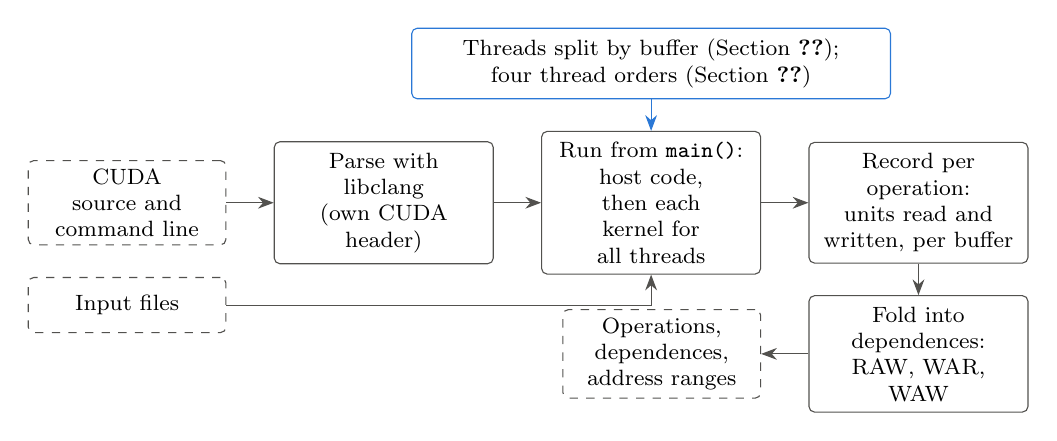
\begin{tikzpicture}[node distance=4mm and 6mm, font=\footnotesize,
  box/.style={draw=muted, rounded corners=2pt, align=center, inner sep=4pt, minimum height=9mm, text width=25mm},
  data/.style={draw=muted, dashed, rounded corners=2pt, align=center, inner sep=3pt, minimum height=7mm,
               text width=23mm},
  arr/.style={-{Stealth[length=2mm]}, color=muted}]
\node[data] (src) {CUDA source and\\command line};
\node[data, below=of src] (input) {Input files};
\node[box, right=of src] (parse) {Parse with libclang\\(own CUDA header)};
\node[box, right=of parse] (run) {Run from \code{main()}:\\host code, then each\\kernel for all threads};
\node[box, right=of run] (events) {Record per operation:\\units read and\\written, per buffer};
\node[box, below=of events] (deps) {Fold into\\dependences:\\RAW, WAR, WAW};
\node[data, left=of deps] (out) {Operations,\\dependences,\\address ranges};
\draw[arr] (src) -- (parse);
\draw[arr] (parse) -- (run);
\draw[arr] (input.east) -| (run.south);
\draw[arr] (run) -- (events);
\draw[arr] (events) -- (deps);
\draw[arr] (deps) -- (out);
\node[box, above=of run, text width=58mm, minimum height=7mm, draw=pblue] (mech)
  {Threads split by buffer (\secref{sec:split}); four thread orders (\secref{sec:schedules})};
\draw[arr, color=pblue] (mech) -- (run);
\end{tikzpicture}
\caption{The steps of the interpreter. Nothing runs on the GPU.}
\label{fig:overview}
\end{figure}

\subsection{Running the host program}
\label{sec:host}

The host part of a CUDA program is ordinary C++, and the interpreter runs it the way \memprint{}'s C++ interpreter
does~\cite{memprintGeneralization}. Every allocation, global variable and the stack is a memory \term{object}. A
pointer is a pair of an object and a byte offset into it. The interpreter keeps the integer value stored in every
4-byte unit of every object, and remembers which units hold pointers and to which object they point. As a result,
when the program reads a graph from a file into an array and later indexes another array with an element of it,
the interpreter knows the index. Floating-point values in memory are not kept, and a value the interpreter does
not know is marked unknown rather than guessed.

Device memory fits into the same scheme. Each \code{cudaMalloc} creates a new object of kind \emph{device}, and
each \code{\_\_device\_\_} or \code{\_\_constant\_\_} variable is an object as well. A \code{cudaMemcpy} copies the
stored values, and the pointer information, from one object to the other, so an index array built on the host and
copied to the GPU keeps its contents, and a table of device pointers built on the host still points to the right
buffers after the copy. A \code{cudaMemset} stores its value in the filled units.

A loop on the host that issues GPU work runs one iteration at a time, in program order. The interpreter otherwise
runs short counted loops as one step over all iterations (\secref{sec:kernels}), and we changed it so that an
allocation, copy or fill inside such a loop is carried out once per iteration, because each iteration creates a
different buffer or a different operation.

\subsection{Running a kernel: all threads at once}
\label{sec:kernels}

A kernel launch runs the kernel's body once, for all of its threads together. Every variable of the kernel holds
an array with one value per thread, and every statement is carried out for all threads before the next statement
starts. \memprint{}'s interpreter uses the same representation to run all iterations of a loop at once, and for a
kernel the threads take the place of the iterations. The thread's \code{threadIdx.x} is an array $0, 1, 2,
\ldots$; an expression such as \code{blockIdx.x * blockDim.x + threadIdx.x} is computed for all threads with one
array operation; and \code{edges[i]}, where \code{i} differs per thread, loads one element per thread from the
stored values of the object \code{edges} points to.

A branch splits the threads. The interpreter evaluates the condition for every thread, runs the branch only for
the threads where it holds, and merges the variables of the two groups afterwards. A loop whose trip count differs
per thread runs until no thread continues, and a thread that returns from the kernel stops taking part. In this
way every thread follows its own control path, decided by the values it loaded.

We call this order of execution \term{lockstep}: statement by statement, all threads at a time. Lockstep is one
order in which the GPU could legally run the threads of a kernel that has no data races, because the GPU guarantees
nothing about the relative progress of threads between barriers. A barrier, \code{\_\_syncthreads()}, has no work
to do in lockstep, since every thread has already reached it when the statement before it finishes. Each block has
its own copy of the kernel's \code{\_\_shared\_\_} arrays. Atomic operations to the same address from different
threads take effect one after another in thread order, and each thread receives the value that was there before
its own update, as on the GPU. The interpreter runs the blocks of a large grid in groups of at most $2^{18}$ threads
to bound its memory use.

\subsection{Recording what each operation touches}
\label{sec:events}

Every operation records, per object and per byte, whether it read the byte and whether it wrote it. A kernel
records every load and store that its threads carry out, a copy records the bytes it reads at the source and writes
at the destination, and a fill records the bytes it writes. The interpreter also records the host code between two
operations as an operation of its own, which a tool can ignore; the evaluation leaves it out.

A record has two further marks. The first says whether the access is only possible, which is the case when the
interpreter could not compute the access exactly. An address it could not compute covers the whole object it
points into, and an access under a branch whose condition is unknown is recorded but marked as possible. An access
through a pointer whose object is unknown is recorded as a possible access to every device buffer. The second mark
says whether the access is data-dependent (\secref{sec:background}). The interpreter decides this from the source
code before the program runs, by marking every value that is loaded from memory, or computed from such a value, or
assigned under a condition that is, and repeating until nothing changes. An access whose address or whose enclosing
conditions use a marked value is data-dependent, and so is every access of a launch that the host issued from a
loop whose condition depends on device data, such as a loop that runs until the GPU reports that nothing changed.

\subsection{From touched bytes to dependences}
\label{sec:deps}

The operations are folded into dependences in the order they were issued. For every unit of every object the
interpreter keeps the last operation that certainly wrote it, the operations that possibly wrote it since then,
and the operations that read it since then. When the next operation arrives, every unit it reads produces a RAW
dependence on the last writer, every unit it writes produces a WAW dependence on the last writer and a WAR
dependence on each reader, and then the operation's own writes replace the history of those units. A dependence is
certain if both of its accesses are certain, and possible otherwise. The counts of units are summed per
dependence. \figref{fig:example} shows the result for a short program.

\begin{figure}[t]
\centering
\begin{minipage}{0.47\linewidth}
\begin{lstlisting}
init<<<b, t>>>(a, 1.0f, n);
init<<<b, t>>>(b, 2.0f, n);
add<<<b, t>>>(a, b, c, n);    // c = a + b
scale<<<4, 64>>>(c, n);       // c *= 2
cudaMemcpy(h, c, n * 4,
           cudaMemcpyDeviceToHost);
\end{lstlisting}
\end{minipage}\hfill
\begin{minipage}{0.5\linewidth}
\centering
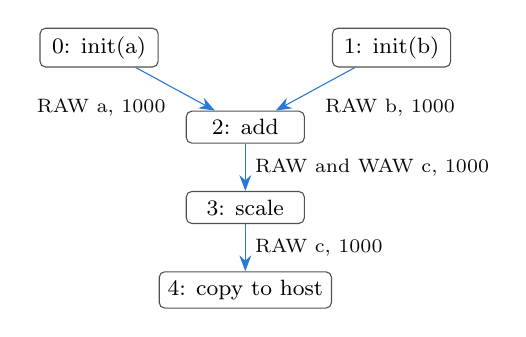
\begin{tikzpicture}[font=\footnotesize, node distance=6mm and 9mm,
  op/.style={draw=muted, rounded corners=2pt, inner sep=3pt, minimum width=15mm, align=center},
  dep/.style={-{Stealth[length=2mm]}, color=pblue}]
\node[op] (i1) {0: init(a)};
\node[op, right=22mm of i1] (i2) {1: init(b)};
\node[op, below=8mm of $(i1)!0.5!(i2)$] (add) {2: add};
\node[op, below=of add] (sc) {3: scale};
\node[op, below=of sc] (cp) {4: copy to host};
\draw[dep] (i1) -- node[below left, pos=0.5, font=\scriptsize, text=ink] {RAW a, 1000} (add);
\draw[dep] (i2) -- node[below right, pos=0.5, font=\scriptsize, text=ink] {RAW b, 1000} (add);
\draw[dep] (add) -- node[right, font=\scriptsize, text=ink] {RAW and WAW c, 1000} (sc);
\draw[dep] (sc) -- node[right, font=\scriptsize, text=ink] {RAW c, 1000} (cp);
\end{tikzpicture}
\end{minipage}
\caption{The operations of \code{chain} with $n=1000$ and the dependences the interpreter reports, with the
number of 4-byte units each passes through. The two \code{init} launches are independent and could run at the
same time. All dependences are certain, and all are needed.}
\label{fig:example}
\end{figure}

\subsection{Threads that use different buffers}
\label{sec:split}

Some kernels choose a buffer, not only an element, from data. \figref{fig:ptrsel} shows a kernel that distributes
elements into one of four buckets, each a separate buffer, through a table of device pointers that the host
copied to the GPU. In lockstep, the statement \code{bucket[k][\ldots] = i} loads one pointer per thread, and the
pointers of different threads point to different buffers. The interpreter's pointer is a pair of one object and
an offset, so it cannot represent ``buffer 0 for these threads and buffer 3 for those''. Before the change
described here, such a pointer became unknown, every write through it became a possible write to every device
buffer, and every dependence from the kernel to the four consumers was only possible.

\begin{figure}[t]
\begin{lstlisting}
__global__ void distribute(const int *keys, int *const *bucket, int *count, int n) {
    int i = blockIdx.x * blockDim.x + threadIdx.x;
    if (i >= n) return;
    int k = keys[i] % 4;
    bucket[k][atomicAdd(&count[k], 1)] = i;   // the buffer itself is chosen by keys[i]
}
\end{lstlisting}
\caption{A kernel that writes each element into one of four buffers, through a table of pointers in device memory
(\code{ptrsel}). The four consumer kernels each read one buffer.}
\label{fig:ptrsel}
\end{figure}

We resolve this by splitting the threads. When a kernel loads pointers from memory and the threads' pointers name
different objects, the interpreter groups the threads by the object their pointer names, and then runs the
statement, and the rest of the enclosing block of code, once for each group, with only that group's threads
active. Inside a group the pointer names one object, so every access through it is exact. After the last group,
the variables of all groups are merged as after a branch. A pointer variable that ends up naming different objects
in different groups becomes unknown at the merge, which is safe.

Running a statement a second time is correct only if its first, interrupted execution changed nothing. The
interpreter therefore counts stores and atomic operations, notes the count when each statement starts, and splits
only if the count is unchanged when the pointer is loaded. If a store already happened, the pointer stays unknown
as before. For \code{bucket[k][atomicAdd(\ldots)]} the split happens, because C++17 evaluates the array expression
\code{bucket[k]} before the index, so the pointer is loaded before the atomic operation~\cite{cppstd17}. A pointer
loaded after an atomic operation in the same statement cannot be split. The interpreter also limits the split to
at most 64 different objects.

\subsection{Kernels whose result depends on thread order}
\label{sec:schedules}

Lockstep is a legal order of execution, but it is not the only one, and for some kernels the bytes touched depend
on the order. The connected-components kernel in \figref{fig:cc} lowers labels in place. Thread $e$ reads the
labels of the two ends of edge $e$ and writes the smaller into the larger with \code{atomicMin}. If another thread
lowered one of those labels earlier in the same launch, thread $e$ reads the new value, otherwise the old one, so
which threads write, and which units, depends on the order. The host repeats the kernel until a launch changes
nothing, so the number of launches depends on the order too. On the GPU, \numCcGpuRuns{} runs of this program took
\numCcGpuRoundsLo{} to \numCcGpuRoundsHi{} rounds, and each of \numCcReps{} traced runs touched different bytes. In lockstep, every
thread reads its labels before any thread of the launch writes one, so no update reaches another thread within the
same round, and the program takes 24 rounds. With lockstep alone, the interpreter reported all of its dependences as
certain, and \numCcLockFalseLo{} to \numCcLockFalseHi{} of them did not occur in a given GPU run
(\secref{sec:eval-cc}).

\begin{figure}[t]
\begin{lstlisting}
__global__ void hook(const int *src, const int *dst, int *label, int *changed, int m) {
    int e = blockIdx.x * blockDim.x + threadIdx.x;
    if (e >= m) return;
    int a = label[src[e]], b = label[dst[e]];   // may see another thread's update, or not
    if (a < b && atomicMin(&label[dst[e]], a) > a) *changed = 1;
    if (b < a && atomicMin(&label[src[e]], b) > b) *changed = 1;
}
\end{lstlisting}
\caption{One round of connected components by label propagation (\code{cc}). The host launches it until
\code{changed} stays zero.}
\label{fig:cc}
\end{figure}

To detect such kernels, the interpreter runs the whole program under several thread orders. All are legal on the
GPU. The first is lockstep. In the other three, each block runs to completion before the next starts, in the
order of block numbers, in reverse order, or in a random order. A later block then sees what earlier blocks wrote.
We match the operations of the runs by their common beginning and their common end, because a loop that runs a
different number of rounds adds or removes operations in the middle of the sequence. The operations before the
loop and the first rounds match from the front, and the operations after the loop match from the back. A dependence stays certain only if
every run has it between matched operations and every run reports it as certain. All other dependences of the
first run, and the dependences that only the other runs have between matched operations, become possible and are
marked as depending on the schedule. A program whose kernels do not depend on the order, such as all three
breadth-first searches in our tests, gives the same dependences under all four orders and loses nothing.

Four orders are a sample of the legal orders, not all of them, so a GPU run can still produce a dependence that
none of the four produced. We return to this in \secref{sec:eval-cc}.

\subsection{What the interpreter cannot know}
\label{sec:unknown}

The interpreter needs the program's input, because the bytes an irregular kernel touches are a function of it.
It does not model floating-point values stored in memory, the values of some library functions (for example
\code{drand48}), or a pointer loaded in a statement after a store. Accesses that depend on such values are
recorded as possible, so the dependences through them are possible too. The \code{maybe} test program checks this
case. A kernel whose result depends on thread order is handled by sampling orders (\secref{sec:schedules}), and a
data race whose outcome no sampled order reproduces is not detected.

\section{Measuring the truth on a GPU}
\label{sec:truth}

To measure the interpreter's accuracy, we need the bytes each operation actually touches on a GPU. We built an
NVBit~\cite{Villa2019NVBit} tool for this. NVBit is a framework that inserts code before chosen machine
instructions of a kernel when the kernel is loaded. Our tool inserts, before every load, store and atomic
operation on global memory, a call that sends the addresses of the 32 threads of the warp, the access size and
whether it reads or writes, together with the number of the current launch, to a buffer that a CPU thread empties.
On the host side the tool intercepts the CUDA driver's functions for allocation, copies, fills and kernel launches,
so it knows every buffer's base address and size and every operation's position. It writes, per operation and
buffer, the ranges of units read and written, in the same format the interpreter can write.

The tool was written against NVBit 1.7 on a machine without a GPU, and it needed three changes to work with NVBit
1.8 and CUDA 13.4. First, the GPU side of the buffer must be flushed explicitly after each launch and at the end,
with a small kernel loaded as a separate module, otherwise the last partly filled buffer, which for a small program
holds all records, is lost. Second, the launch number must be set before the instrumented code is enabled for the
launch, otherwise the records carry a wrong number. Third, the CUDA 13 runtime may launch kernels through
\code{cuLaunchKernelEx}, which the tool must intercept as well. In addition, the interpreter's stand-in CUDA header had to declare the launch function
that clang uses when it finds a recent CUDA installation on the machine.

\paragraph{Comparing two runs.} The traced run's bytes are folded into dependences by the same code as the
interpreter's, so the two sides differ only in which bytes each operation touched. Buffers are matched by the
order of their allocation, and operations by their order. When the two runs issue different numbers of operations,
as \code{cc} does, operations are matched by common beginning and common end as in \secref{sec:schedules}, and a
traced dependence through an unmatched operation counts as missed. We report four scores. \term{Certain precision}
is the share of the interpreter's certain dependences that the traced run has. \term{Recall} is the share of the
traced run's dependences that the interpreter reports, certain or possible. \term{Certain recall} is the share it
reports as certain. \term{Units error} is, over the dependences both have, the summed difference in unit counts
divided by the traced units. We compute the same scores over the needed dependences of each side.

\section{Evaluation}
\label{sec:eval}

\subsection{Setup}
\label{sec:setup}

We ran the GPU programs on an NVIDIA A30 (compute capability 8.0) with driver 610.57, CUDA 13.4 and NVBit 1.8,
and the interpreter on the same machine's CPU, with Python 3.10, NumPy and libclang 18.1. The programs were compiled
with \code{nvcc -O2}. \tabref{tab:programs} lists the \numPrograms{} test programs. They are small, between 22 and
103 lines of code, and each exercises one pattern: regular elementwise kernels, shared memory, scattered writes
through host-built or file-provided indices, atomics, values the interpreter does not model, three versions of
breadth-first search (one kernel per level, Rodinia's two-kernel form with a graph file, and a frontier queue
filled with \code{atomicAdd}), buffers chosen through pointer tables, and connected components. The graphs have
4{,}096 vertices with 1 to 5 random neighbours each. We wrote the programs together with the interpreter, so they
test the patterns it was built for; \secref{sec:limits} discusses what this does not show.

\begin{table}[t]
\centering
\footnotesize
\setlength{\tabcolsep}{4pt}
\begin{tabular}{llrrrr}
\toprule
Program & What it exercises & Lines & Kernels & Operations & Dependences \\
\midrule
\texttt{chain} & elementwise kernels in a chain & 32 & 3 & 5 & 5 \\
\texttt{reduce} & a reduction through shared memory & 39 & 2 & 5 & 4 \\
\texttt{stencil} & a stencil repeated over two buffers & 22 & 1 & 7 & 16 \\
\texttt{scatter} & writes at indices built on the host & 35 & 3 & 6 & 5 \\
\texttt{fileidx} & indices and weights read from files & 41 & 2 & 5 & 6 \\
\texttt{histogram} & atomic updates of bins chosen by the data & 45 & 2 & 10 & 14 \\
\texttt{maybe} & a branch on values the interpreter does not model & 30 & 2 & 4 & 5 \\
\texttt{bfs} & breadth-first search, one kernel per level & 50 & 1 & 49 & 359 \\
\texttt{rodinia\_bfs} & breadth-first search in the style of Rodinia & 103 & 2 & 59 & 609 \\
\texttt{wl\_bfs} & breadth-first search with a frontier queue & 60 & 1 & 56 & 345 \\
\texttt{ptrsel} & a buffer chosen by the data through a pointer table & 35 & 2 & 10 & 21 \\
\texttt{ptrsel2} & pointer fields in structs, pointers in variables & 88 & 4 & 16 & 29 \\
\texttt{symbols} & device and constant variables, symbol copies & 46 & 3 & 8 & 6 \\
\texttt{cc} & connected components, labels lowered in place & 49 & 2 & 76 & 653 \\
\bottomrule
\end{tabular}

\caption{The test programs. Lines counts non-empty, non-comment lines. Operations is the number of kernel launches,
copies and fills the program issues, and dependences the number of dependences on the GPU.}
\label{tab:programs}
\end{table}

\subsection{Accuracy of the dependences}
\label{sec:eval-acc}

\tabref{tab:accuracy} compares the interpreter, run under all four thread orders, with one traced run of each
program. \textit{Every dependence the interpreter reports as certain occurs on the GPU}: the certain precision is
1.00 for all 13 programs, over \numMustTotal{} certain dependences. The interpreter finds every traced dependence of
12 programs, and \numCcRecall{} of those of \code{cc}. In 10 of the 13 programs it reports every dependence as
certain, and the unit counts match exactly.

The three exceptions are the programs built to contain what the interpreter cannot resolve exactly. In
\code{maybe}, a branch on \code{drand48} values makes two dependences possible, and one of them did not occur on
the GPU. In \code{ptrsel2}, one kernel loads its pointer after an atomic operation in the same statement, so its
threads cannot be split (\secref{sec:split}), and its accesses are possible accesses to every device buffer; the
other three kernels of the program are exact. In \code{cc}, the dependences of rounds whose touched bytes depend on
thread order are possible (\secref{sec:eval-cc}).

\begin{table*}[t]
\centering
\footnotesize
\setlength{\tabcolsep}{4pt}
\begin{tabular}{lrrrrrrrrrr}
\toprule
 & \multicolumn{7}{c}{Dependences} & \multicolumn{3}{c}{Address ranges} \\
\cmidrule(lr){2-8} \cmidrule(lr){9-11}
Program & Certain & Possible & \shortstack{Certain\\precision} & Recall & \shortstack{Certain\\recall} & \shortstack{Needed cert.\\precision} & \shortstack{Needed\\recall} & \shortstack{Exact\\sets} & \shortstack{Unit\\precision} & \shortstack{Unit\\recall} \\
\midrule
\texttt{chain} & 5 & 0 & 1.00 & 1.00 & 1.00 & 1.00 & 1.00 & 8/8 & 1.00 & 1.00 \\
\texttt{reduce} & 4 & 0 & 1.00 & 1.00 & 1.00 & 1.00 & 1.00 & 7/7 & 1.00 & 1.00 \\
\texttt{stencil} & 16 & 0 & 1.00 & 1.00 & 1.00 & 1.00 & 1.00 & 11/11 & 1.00 & 1.00 \\
\texttt{scatter} & 5 & 0 & 1.00 & 1.00 & 1.00 & 1.00 & 1.00 & 9/9 & 1.00 & 1.00 \\
\texttt{fileidx} & 6 & 0 & 1.00 & 1.00 & 1.00 & 1.00 & 1.00 & 8/8 & 1.00 & 1.00 \\
\texttt{histogram} & 14 & 0 & 1.00 & 1.00 & 1.00 & 1.00 & 1.00 & 17/17 & 1.00 & 1.00 \\
\texttt{maybe} & 3 & 2 & 1.00 & 1.00 & 0.60 & 1.00 & 1.00 & 7/8 & 0.94 & 1.00 \\
\texttt{bfs} & 359 & 0 & 1.00 & 1.00 & 1.00 & 1.00 & 1.00 & 108/108 & 1.00 & 1.00 \\
\texttt{rodinia\_bfs} & 609 & 0 & 1.00 & 1.00 & 1.00 & 1.00 & 1.00 & 195/195 & 1.00 & 1.00 \\
\texttt{wl\_bfs} & 345 & 0 & 1.00 & 1.00 & 1.00 & 1.00 & 1.00 & 172/172 & 1.00 & 1.00 \\
\texttt{ptrsel} & 21 & 0 & 1.00 & 1.00 & 1.00 & 1.00 & 1.00 & 25/25 & 1.00 & 1.00 \\
\texttt{ptrsel2} & 23 & 34 & 1.00 & 1.00 & 0.79 & 1.00 & 0.90 & 31/49 & 0.57 & 1.00 \\
\texttt{cc} & 240 & 466 & 1.00 & 0.98 & 0.35 & 1.00 & 1.00 & 151/170 & 0.99 & 0.99 \\
\bottomrule
\end{tabular}

\caption{The interpreter against one traced run per program. Certain and Possible count the interpreter's
dependences. Precision and recall are defined in \secref{sec:truth}; ``Needed'' columns score only the needed
dependences of each side. The address-range columns compare, for every operation, buffer, and read or write, the
set of units touched: Exact sets counts how many of these sets are identical, and unit precision and recall are
the shares of the interpreter's units the GPU touched and of the GPU's units the interpreter reported.}
\label{tab:accuracy}
\end{table*}

\subsection{Dependences through data-dependent addresses and branches}
\label{sec:eval-data}

\tabref{tab:datadep} restricts the comparison to dependences between two kernels that pass through bytes touched
by an indirect access or under a data-dependent branch, the dependences a compiler cannot determine. There are
\numDataDeps{} of them across the programs. The interpreter reports \numDataMust{} as certain, and all of these
occur on the GPU. In the three breadth-first searches, every one of the \numBfsDeps{} such dependences is
certain and correct, including those through the frontier queue of \code{wl\_bfs}, whose slots threads claim with
\code{atomicAdd} in an order that differs between runs. The order changes which vertex lands in which slot, but
not the set of slots written or the set of vertices whose distances the next level reads, so the dependences
between launches do not change. In \code{ptrsel}, the dependence of each consumer on the bucket it reads is
certain, with the exact number of elements, and the consumer of the bucket that stays empty has no dependence on the
producer. The remaining dependences of this kind are the possible ones of \code{maybe}, \code{ptrsel2} and \code{cc}
described above.

\begin{table}[t]
\centering
\small
\begin{tabular}{lrrrrr}
\toprule
Program & \shortstack{Between\\kernels} & \shortstack{Through data-\\dependent bytes} & \shortstack{Reported\\certain} & \shortstack{Certain and\\in the trace} & \shortstack{In the trace\\(any)} \\
\midrule
\texttt{scatter} & 1 & 1 & 1 & 1 & 1 \\
\texttt{fileidx} & 1 & 1 & 1 & 1 & 1 \\
\texttt{histogram} & 1 & 1 & 1 & 1 & 1 \\
\texttt{maybe} & 2 & 1 & 0 & 0 & 1 \\
\texttt{bfs} & 233 & 233 & 233 & 233 & 233 \\
\texttt{rodinia\_bfs} & 454 & 454 & 454 & 454 & 454 \\
\texttt{wl\_bfs} & 181 & 181 & 181 & 181 & 181 \\
\texttt{ptrsel} & 6 & 6 & 6 & 6 & 6 \\
\texttt{ptrsel2} & 22 & 11 & 2 & 2 & 6 \\
\texttt{cc} & 1152 & 538 & 120 & 120 & 445 \\
\midrule
Total & 2068 & 1427 & 999 & 999 & 1329 \\
\bottomrule
\end{tabular}

\caption{Dependences between two kernels (copies and fills excluded), and among them those through bytes reached by
an indirect access or under a data-dependent branch. The last two columns count how many of the latter the traced
run has. Programs with none are omitted.}
\label{tab:datadep}
\end{table}

\paragraph{Address ranges.} The right part of \tabref{tab:accuracy} compares the units each operation touched,
not only the dependences. For 11 programs every set of units is identical to the GPU's. The interpreter's sets
are larger only where it reports possible accesses: \code{maybe} (512 units possibly written, 254 written),
\code{ptrsel2} (the kernel whose pointer could not be split covers every buffer) and \code{cc}.

\paragraph{How much the exact ranges add.} In our programs, most kernels touch all or most of every buffer they
use, so tracking whole buffers instead of exact units gives the same dependences for 10 of the 13 programs
(\tabref{tab:granularity}). Exact ranges matter in \code{ptrsel} and \code{ptrsel2}, where several kernels touch
disjoint parts of shared buffers, and they remove one false pair in \code{scatter} and \code{wl\_bfs}. The test
programs therefore show that the interpreter finds the exact bytes, but not that exact bytes are needed; programs
whose kernels partition buffers, such as blocked matrix factorisations, would show that.

\begin{table}[t]
\centering
\small
\begin{tabular}{lrrrrrr}
\toprule
 & \multicolumn{2}{c}{Exact units} & \multicolumn{2}{c}{One interval} & \multicolumn{2}{c}{Whole allocation} \\
\cmidrule(lr){2-3} \cmidrule(lr){4-5} \cmidrule(lr){6-7}
Program & Pairs & Needed & Pairs & Needed & Pairs & Needed \\
\midrule
\texttt{chain} & 5 & 4 & 5 & 4 & 5 & 4 \\
\texttt{reduce} & 4 & 4 & 4 & 4 & 4 & 4 \\
\texttt{stencil} & 17 & 6 & 17 & 6 & 17 & 6 \\
\texttt{scatter} & 6 & 5 & 7 & 5 & 7 & 5 \\
\texttt{fileidx} & 5 & 4 & 5 & 4 & 5 & 4 \\
\texttt{histogram} & 13 & 9 & 13 & 9 & 13 & 9 \\
\texttt{maybe} & 4 & 3 & 4 & 3 & 4 & 3 \\
\texttt{bfs} & 916 & 48 & 916 & 48 & 916 & 48 \\
\texttt{rodinia\_bfs} & 1009 & 69 & 1009 & 69 & 1009 & 69 \\
\texttt{wl\_bfs} & 1185 & 55 & 1190 & 55 & 1191 & 55 \\
\texttt{ptrsel} & 17 & 13 & 18 & 13 & 21 & 9 \\
\texttt{ptrsel2} & 26 & 18 & 26 & 18 & 27 & 15 \\
\texttt{symbols} & 6 & 4 & 6 & 4 & 6 & 4 \\
\texttt{cc} & 2139 & 72 & 2139 & 72 & 2139 & 72 \\
\bottomrule
\end{tabular}

\caption{Pairs of operations that conflict in the traced run (both touch a unit and one writes it), and the needed
pairs among them, when each operation's touched units are taken exactly, as one interval per buffer, or as the
whole buffer.}
\label{tab:granularity}
\end{table}

\subsection{Kernels whose result depends on thread order}
\label{sec:eval-cc}

\figref{fig:cc-rounds} shows how many rounds \code{cc} takes. On the GPU, \numCcPlain{} plain runs and
\numCcReps{} runs under NVBit took between \numCcGpuRoundsLo{} and \numCcGpuRoundsHi{} rounds. The interpreter's
orders took \numCcInterpRoundsLo{} to \numCcInterpRoundsHi{} rounds. Lockstep takes the most rounds, because no
label update reaches another thread within a round. Running blocks one after another lets labels flow from earlier
blocks to later ones within a round, which takes fewer rounds. The GPU, which runs many blocks at once but not all
of them, lies between the two, inside the interpreter's range.

\begin{figure}[t]
\centering
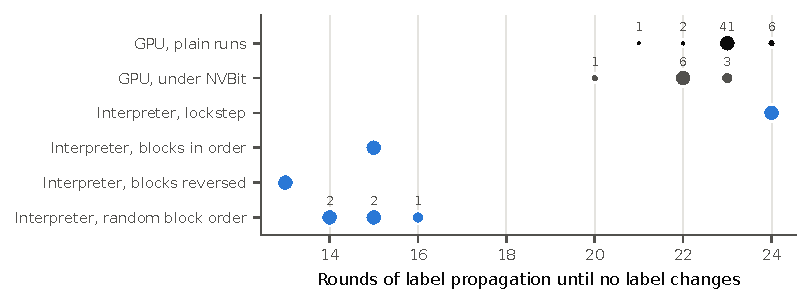
\includegraphics[width=0.75\linewidth]{figures/cc_rounds}
\caption{Rounds of \code{cc} until no label changes, on the GPU and in the interpreter. Each dot is a round count,
its size and the number above it give how many runs produced it. The random order was run with five seeds.}
\label{fig:cc-rounds}
\end{figure}

\figref{fig:cc-scores} scores the interpreter against each of the \numCcReps{} traced runs. With lockstep alone,
the interpreter reports all of its dependences as certain, and \numCcLockPrecLo{} to \numCcLockPrecHi{} of them
occur in a given run, so the rest are false. With the four orders merged, the certain precision is 1.00 against
every run, and the interpreter reports \numCcMustRecallLo{} to \numCcMustRecallHi{} of each run's dependences as
certain and \numCcRecallLo{} to \numCcRecallHi{} as certain or possible. The certain ones are mostly those of the
early rounds and of the setup, which every order shares. A run's dependences that the interpreter misses come
from orders that none of the four produced, for example a label written in one round and next overwritten three
rounds later.

\begin{figure}[t]
\centering
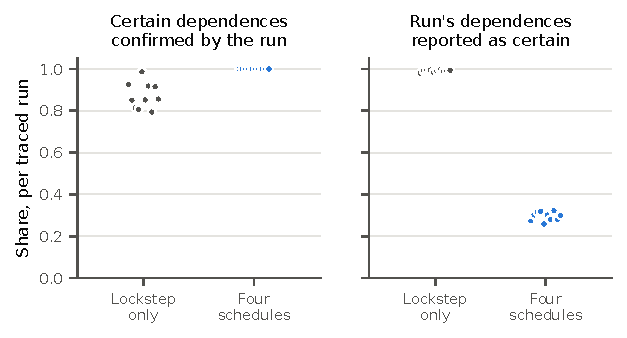
\includegraphics[width=0.62\linewidth]{figures/cc_scores}
\caption{\code{cc} against each traced run: the share of the interpreter's certain dependences that the run has
(left), and the share of the run's dependences that the interpreter reports as certain (right). Lockstep alone
reports false certain dependences, and the four orders together do not.}
\label{fig:cc-scores}
\end{figure}

\subsection{What each mechanism contributes}
\label{sec:eval-ablation}

\tabref{tab:ablation} turns each of the two mechanisms off in turn. Without splitting threads by buffer, every
dependence through the buckets of \code{ptrsel} becomes possible, so only \numPtrselNoSplitMust{} of the 21
traced dependences are reported as certain and only half of the needed ones; in \code{ptrsel2}, certain recall
falls from 0.79 to 0.55 and certain recall of the needed dependences from 0.81 to 0.10. Recall stays at 1.00,
because the unknown pointer makes the accesses possible accesses to every buffer, which includes the right one.
Without the extra thread orders, \code{cc} reports false certain dependences, as \secref{sec:eval-cc} showed.

\begin{table}[t]
\centering
\footnotesize
\setlength{\tabcolsep}{4pt}
\begin{tabular}{llrrrrrrr}
\toprule
Program & Interpreter & Certain & Possible & \shortstack{Certain\\precision} & Recall & \shortstack{Certain\\recall} & \shortstack{Needed cert.\\recall} & \shortstack{Units\\error} \\
\midrule
\texttt{ptrsel} & Full interpreter & 21 & 0 & 1.00 & 1.00 & 1.00 & 1.00 & 0.00 \\
\texttt{ptrsel} & Without thread splitting & 10 & 22 & 1.00 & 1.00 & 0.48 & 0.50 & 0.00 \\
\addlinespace
\texttt{ptrsel2} & Full interpreter & 21 & 36 & 1.00 & 1.00 & 0.72 & 0.81 & 0.07 \\
\texttt{ptrsel2} & Without thread splitting & 4 & 105 & 1.00 & 1.00 & 0.14 & 0.10 & 0.47 \\
\addlinespace
\texttt{cc} & Full interpreter & 32 & 1058 & 1.00 & 1.00 & 0.05 & 0.17 & 0.15 \\
\texttt{cc} & Lockstep schedule only & 703 & 0 & 0.85 & 0.99 & 0.99 & 0.96 & 0.06 \\
\bottomrule
\end{tabular}

\caption{The interpreter with one mechanism turned off, against the same traced runs as \tabref{tab:accuracy}.}
\label{tab:ablation}
\end{table}

\subsection{Overhead}
\label{sec:eval-overhead}

The interpreter's cost is its run time on the CPU. \figref{fig:overhead} and \tabref{tab:overhead} compare it with
the program's own run on the GPU and with the run under the NVBit tool, for six programs at three input sizes
each. The GPU runs take \numNativeLo{} to \numNativeHi{} seconds, and almost all of that time is the start-up of
the CUDA runtime, because at these sizes the kernels themselves take milliseconds. Against the whole GPU run, the
interpreter in lockstep takes \numOverheadLo{} to \numOverheadHi{} times as long, and the NVBit tool \numNvbitLo{}
to \numNvbitHi{} times. Against the kernels alone, the interpreter is several orders of magnitude slower, as
expected from simulating every thread in Python on one CPU core.

\textit{Most of the interpreter's time is spent in host code, not in kernels.} The ``In kernels'' column of
\tabref{tab:overhead} gives the share of the time spent running kernels. The kernels of \code{chain}, with
\numChainThreads{} GPU threads, take \numChainKernelS{} seconds, and those of \code{rodinia\_bfs}, with
\numRbfsThreads{} threads, take less than one second, so \code{rodinia\_bfs} as a whole takes \numRbfsLockS{}
seconds, against \numRbfsNvbitS{} seconds under NVBit. The time spent in kernels alone is \numKernelRatioLo{} to
\numKernelRatioHi{} times the whole GPU run, with a median of \numKernelRatioMedian{}. The programs that take
longest, \code{wl\_bfs} (\numWlbfsLockS{} seconds, of which \numWlbfsKernelS{} in kernels) and \code{bfs}
(\numBfsLockS{} seconds, of which \numBfsKernelS{} in kernels), spend up to \numHostShareMax{} of their time in host
loops that carry a value from one iteration to the next. These loops are the random-number generator that builds
the graph in \code{wl\_bfs} and \code{cc}, and a running maximum over the result in \code{bfs}. The interpreter runs
all iterations of a loop at once only when the iterations do not depend on each other, so it runs these loops one
iteration at a time, at about a millisecond per iteration. Such loops belong to the test harness here, not to the
computation on the GPU, but real programs contain them as well, for example when they read or generate their input.

Running all four thread orders costs \numScheduleLo{} to \numScheduleHi{} times as much as lockstep alone
(\numScheduleCost{} on average). Where host code dominates, the cost is close to four times, because each order runs
the host code once more. Where kernels dominate, the orders that run one block at a time cost much more than
lockstep, because they carry out every statement once per block instead of once per group of up to $2^{18}$ threads.
A tool could run the extra orders only for kernels that read memory that other threads of the same launch write,
which is where the order can change the result. We have not done so.


\begin{figure}[t]
\centering
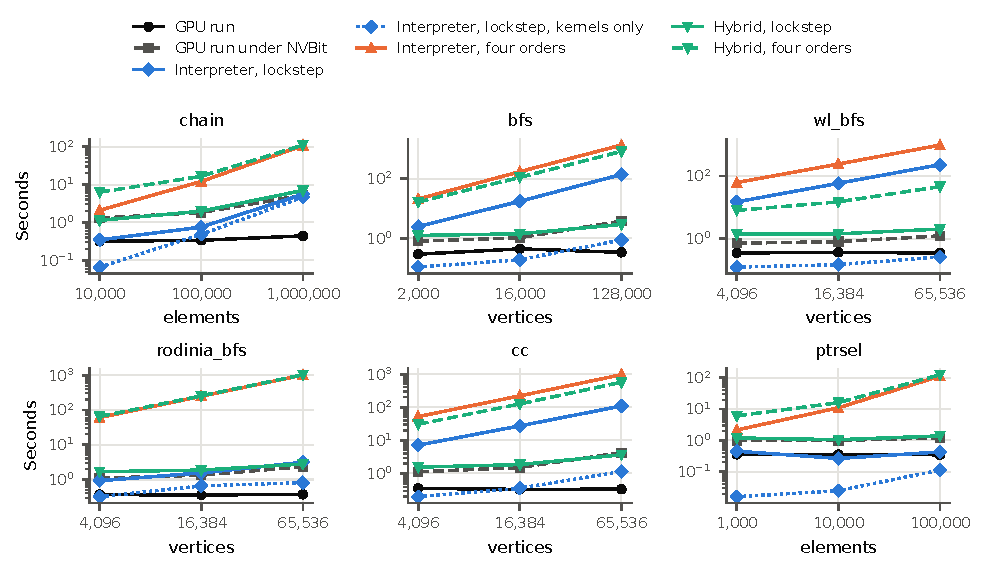
\includegraphics[width=\linewidth]{figures/overhead}
\caption{Wall-clock time against input size, both axes logarithmic: the program on the GPU (CUDA start-up
included), the program under the NVBit tool, the interpreter in lockstep, the part of that time spent running
kernels, and the interpreter under all four thread orders together.}
\label{fig:overhead}
\end{figure}

\begin{table*}[t]
\centering
\footnotesize
\setlength{\tabcolsep}{4pt}
\begin{tabular}{lrrrrrrrrr}
\toprule
 & & & & \multicolumn{2}{c}{GPU (s)} & \multicolumn{4}{c}{Interpreter} \\
\cmidrule(lr){5-6} \cmidrule(lr){7-10}
Program & Input & \shortstack{GPU\\threads} & Operations & Run & \shortstack{Under\\NVBit} & \shortstack{Lockstep\\(s)} & \shortstack{In\\kernels} & \shortstack{Four\\schedules (s)} & \shortstack{Lockstep /\\GPU run} \\
\midrule
\texttt{chain} & 10,000 & 30,592 & 5 & 0.33 & 1.25 & 0.14 & 33\% & 1.7 & 0.4 \\
\texttt{chain} & 100,000 & 300,544 & 5 & 0.36 & 1.54 & 0.54 & 77\% & 15.4 & 1.5 \\
\texttt{chain} & 1,000,000 & 3,000,448 & 5 & 0.34 & 4.74 & 4.62 & 86\% & 166.5 & 13.5 \\
\addlinespace
\texttt{bfs} & 2,000 & 30,720 & 49 & 0.36 & 0.70 & 2.14 & 4\% & 11.1 & 6.0 \\
\texttt{bfs} & 16,000 & 288,000 & 58 & 0.34 & 0.88 & 15.48 & 1\% & 85.6 & 46.1 \\
\texttt{bfs} & 128,000 & 2,816,000 & 70 & 0.36 & 2.86 & 121.90 & 1\% & 690.3 & 341.4 \\
\addlinespace
\texttt{rodinia\_bfs} & 4,096 & 106,496 & 59 & 0.35 & 1.06 & 0.66 & 47\% & 6.9 & 1.9 \\
\texttt{rodinia\_bfs} & 16,384 & 524,288 & 71 & 0.37 & 1.23 & 1.10 & 38\% & 25.0 & 3.0 \\
\texttt{rodinia\_bfs} & 65,536 & 2,228,224 & 75 & 0.36 & 2.19 & 2.77 & 26\% & 106.3 & 7.7 \\
\addlinespace
\texttt{wl\_bfs} & 4,096 & 5,120 & 56 & 0.36 & 0.81 & 14.08 & 1\% & 55.4 & 39.2 \\
\texttt{wl\_bfs} & 16,384 & 16,128 & 59 & 0.37 & 0.82 & 54.64 & 0\% & 218.7 & 146.9 \\
\texttt{wl\_bfs} & 65,536 & 60,288 & 71 & 0.34 & 1.21 & 214.14 & 0\% & 871.0 & 624.3 \\
\addlinespace
\texttt{cc} & 4,096 & 102,400 & 76 & 0.36 & 1.05 & 6.46 & 3\% & 28.3 & 18.1 \\
\texttt{cc} & 16,384 & 409,600 & 76 & 0.32 & 1.37 & 24.92 & 1\% & 112.2 & 77.2 \\
\texttt{cc} & 65,536 & 1,835,008 & 85 & 0.33 & 3.69 & 99.95 & 1\% & 459.5 & 305.7 \\
\addlinespace
\texttt{ptrsel} & 1,000 & 5,120 & 10 & 0.33 & 0.95 & 0.11 & 13\% & 0.6 & 0.3 \\
\texttt{ptrsel} & 10,000 & 50,560 & 10 & 0.33 & 0.95 & 0.12 & 18\% & 2.6 & 0.4 \\
\texttt{ptrsel} & 100,000 & 500,480 & 10 & 0.31 & 1.09 & 0.26 & 41\% & 24.2 & 0.8 \\
\bottomrule
\end{tabular}

\caption{Run times. GPU threads is the total number of threads of all launches. The GPU columns are wall-clock
times of the whole program, CUDA start-up included (median of three runs). ``In kernels'' is the share of the
lockstep interpreter's time spent running kernels; the rest runs host code. The last column divides the lockstep
interpreter's time by the GPU run.}
\label{tab:overhead}
\end{table*}

\subsection{Before the input is known}
\label{sec:eval-input}

The interpreter needs the input. To see what depends on the input and what does not, we ran \code{rodinia\_bfs}
on three random graphs (\tabref{tab:patterns}). The searches took 51 to 63 operations and produced 417 to 656
dependences, and only 48 dependences have the same operations and units in all three graphs, most of them
through the one-unit flag that the host copies back after every round. The
exact bytes are therefore a property of the input. We then describe each dependence by a \term{pattern}: the names
of its two operations, its kind, its buffer, and how many operations apart they are, for example ``\code{expand}
then \code{commit} one operation later, RAW through \code{updating}''. All 24 patterns of the needed dependences are
the same for the three graphs. The structure of the dependences is therefore a property of the program, and only
the number of rounds and the units are a property of the input. A tool that must decide before the input is known
could use the patterns, and refine them with the interpreter once the input is available. We have not built such
a tool. Run without the input, the interpreter today stops after one round of the search, because the loop's exit
condition comes from the GPU and is unknown, and it reports \numNoInputPatterns{} of the \numNoInputPatternsOf{}
patterns that connect operations at most six apart, nearly all of them as possible.

\begin{table}[t]
\centering
\small
\setlength{\tabcolsep}{4pt}
\begin{tabular}{lrrrrrrr}
\toprule
Input & Vertices & Edges & Operations & Dependences & Needed & \shortstack{Same bytes\\in all graphs} & \shortstack{Needed patterns\\in all graphs} \\
\midrule
graph A & 4,096 & 12,184 & 59 & 610 & 155 & 48 & 24/24 \\
graph B & 4,096 & 12,289 & 63 & 656 & 168 & 48 & 24/24 \\
graph C & 8,192 & 41,222 & 51 & 417 & 129 & 48 & 24/24 \\
no input & -- & -- & 11 & 56 & 37 & -- & 15/22 \\
\bottomrule
\end{tabular}

\caption{\code{rodinia\_bfs} on three graphs. ``Same bytes in all graphs'' counts dependences with the same
operations, kind, buffer and unit count in all three. A pattern is a dependence without its position: the names of
its operations, kind, buffer and distance in operations.}
\label{tab:patterns}
\end{table}

\section{Related work}
\label{sec:related}

\paragraph{Static analysis of GPU kernels.} Compilers determine the dependences of loops and kernels whose
addresses are affine functions of loop indices with the polyhedral model~\cite{Feautrier1991Dataflow,grosser2012polly},
but an address read from memory falls outside that model. GPUVerify~\cite{Betts2012GPUVerify} proves that a kernel
is free of data races for all inputs, and GKLEE~\cite{Li2012GKLEE} explores a kernel's behaviour with symbolic
inputs. Both reason about one kernel and treat memory contents as arbitrary, so neither tells which bytes a kernel
touches on a given input, and neither relates one launch to the next. Our interpreter answers the latter question,
for one input.

\paragraph{Dynamic analysis.} NVBit~\cite{Villa2019NVBit} and race detectors such as
BARRACUDA~\cite{Eizenberg2017Barracuda} observe the accesses of a running program on the GPU, as our ground-truth
tool does. They give the exact bytes of one run, but only by running the program on the GPU with instrumentation,
and only after the fact. The interpreter gives the same information before the program runs on the GPU, from the
source and the input.

\paragraph{Inspector and executor.} Runtime parallelisation of irregular loops runs an \term{inspector} that reads
the index arrays to compute the loop's dependences, and then an \term{executor} that runs the loop in an order that
respects them~\cite{Saltz1991Inspector}. The interpreter is an inspector for a whole CUDA program. For accesses
whose indices come only from the input, an inspector can be cheap, but in the breadth-first searches the indices
depend on values earlier kernels computed, so finding the dependences means computing those values, which the
interpreter does.

\paragraph{Dependence-driven GPU scheduling.} Wireframe~\cite{Abdolrashidi2017Wireframe} and
BlockMaestro~\cite{Abdolrashidi2021BlockMaestro} run GPU work from a dependence graph between thread blocks of
consecutive kernels, and CUDA graphs~\cite{cudaguide} let the programmer state dependences between operations.
They need the dependences as input. BlockMaestro derives them from the kernels' memory accesses when these are
regular; the interpreter could supply them for irregular kernels when the input is known.

\paragraph{Irregular GPU benchmarks.} Rodinia~\cite{Che2009Rodinia}, Pannotia~\cite{Che2013Pannotia}, the
LonestarGPU programs~\cite{Burtscher2012Irregular} and Gunrock~\cite{Wang2016Gunrock} contain the patterns of our
test programs: frontier arrays, frontier queues filled with atomics, and label propagation. We have not yet run the
interpreter on these suites.

\section{Limitations}
\label{sec:limits}

A limitation of the evaluation is that the test programs are small and were written together with the
interpreter, which means that they show that the mechanisms work on the patterns they target, not how often real
programs contain patterns the interpreter does not support. Unmodified benchmark suites will use library calls,
templates, streams and larger inputs that the tests do not.

A limitation of the interpreter is that it needs the program's input, which means that its exact results are for
that input only (\secref{sec:eval-input}).

A limitation of the thread orders is that they are four samples of the legal orders, which means that a GPU run of
a kernel whose result depends on the order can produce dependences the interpreter misses (\numCcMissLo{} to
\numCcMissHi{} of the traced dependences of \code{cc}).

A limitation of splitting threads is that it applies only to a pointer loaded before any store in its statement,
which means that a pointer loaded after an atomic operation in the same statement still makes every access through
it a possible access to every buffer.

A limitation of the cost is that the interpreter simulates every GPU thread on one CPU core in Python, which means
that its run time grows with the number of threads and with sequential host loops, and that the three extra thread
orders cost more than lockstep because they run one block at a time (\secref{sec:eval-overhead}).

\section{Conclusion}
\label{sec:conclusion}

We showed that the memory dependences between the operations of a CUDA program, including those that pass through
bytes chosen by data, can be found before the program runs on the GPU, by interpreting its source on the CPU with
its input. Running all threads of a kernel at once as arrays keeps the cost proportional to the work of the
kernels, splitting threads by the buffer their pointers name makes accesses through pointer tables exact, and
running several legal thread orders keeps the reported certain dependences correct when a kernel's result depends
on the order. Against an NVIDIA A30, every certain dependence the interpreter reported occurred, and it missed
dependences only in a kernel whose behaviour changed from run to run. The next steps are to run the interpreter on
unmodified graph benchmarks at full input sizes, and to derive the input-independent pattern of dependences
without the input.

\bibliographystyle{plain}
\bibliography{references}

\end{document}
